\documentclass{ctuthesis}
\usepackage{lingmacros}
\usepackage{tree-dvips}
\usepackage{graphicx}
\usepackage{caption}
\usepackage{subcaption}
\usepackage{float}
\usepackage{gensymb}
\usepackage{amsfonts} 
\usepackage{amsmath}
\usepackage[utf8]{inputenc}
\newcommand{\ts}{\textsuperscript}
\usepackage{listings}
\usepackage{color}

\definecolor{dkgreen}{rgb}{0,0.6,0}
\definecolor{gray}{rgb}{0.5,0.5,0.5}
\definecolor{mauve}{rgb}{0.58,0,0.82}
\graphicspath{ {./resources/} }

\lstset{frame=tb,
  language=Python,
  aboveskip=3mm,
  belowskip=3mm,
  showstringspaces=false,
  columns=flexible,
  basicstyle={\small\ttfamily},
  numbers=none,
  numberstyle=\tiny\color{gray},
  keywordstyle=\color{blue},
  commentstyle=\color{dkgreen},
  stringstyle=\color{mauve},
  breaklines=true,
  breakatwhitespace=true,
  tabsize=3
}

\ctusetup{
	xdoctype = B,
	xfaculty = F3,
	mainlanguage = english,
	titlelanguage = english,
	title-english = {Human tracking using computer vision with a data output},
	title-czech = {Trackování lidí pomocí počítačového vidění s datovým výstupem},
	department-english = {Department of Computer Graphics and Interaction},
	author = {Vilém Jonák},
	supervisor = {MgA. Vojtěch Leischner},
	supervisor-address = {Karlovo náměstí 13,\\
	  12000 Praha 2},
    keywords-czech = {prostorové audio, trackování lidí, počítačové vidění, YOLO, DeepSORT, Resonance Audio},
	keywords-english = {spatial audio, human tracking, computer vision, YOLO, DeepSORT, Resonance Audio},
	day = 23
	month = 3,
	year = 2022
}

\ctuprocess

\begin{abstract-english}
We are trying to develop an interactive installation where our program will track people from the top view and send an appropriate spatial audio mix to their headset. This audio is rendered with the Resonance Audio engine. Our main problem is remembering specific detected people, so if the neural network loses them and then again finds them, their id would not change. Minimizing this mismatch rate is crucial for the correct function of the whole installation. Human recognizing and tracking is a shared computer vision task. Many solutions exist that differ according to particular use cases. We needed to solve how to track people from the top view, assign them an id, and remember them with the given id. We decided to use the convolutional neural network YOLOv4 (You Only Look Once) for recognizing people on the frame received from a camera and the DeepSORT algorithm. YOLO differs from other networks. It is trying to predict bounding boxes alongside the class probabilities for these boxes. It is a single network \cite{6}. The DeepSORT algorithm remembers the movement of the detected object and tries to predict a future trajectory for the following frames. This paper's objective is not to create a tracking algorithm but to decide which one will suit our use case and extend it.  TODO{VYSLEDKY}
\end{abstract-english}

\begin{abstract-czech}
Snažíme se vyvinout interaktivní instalaci , ve které bude náš program trackovat lidi shora a posílat do jejich sluchátek prostorový audio mix. Toto audio je vytořeno pomocí enginu Resonance Audio. Hlavní problém, kterému čelíme, je jak si zapamtovávat detekované lidi tak, aby po tom co je neurální síť ztratí a znovu najde, se jejich identifikační číslo nezměnilo. Minimalizovat tuto chybu je zásadní pro optimální fungování instalace, kterou vytváříme.
Rozpoznávání a trackování lidí je běžná úloha počítačového vidění. Existuje mnoho řešení, která se liší podle případu použití. Potřebovali jsme vyřešit jak trackovat lidi z pohledu shora, přiřadit jim identifikační číslo, a zapamtovat si je s ním. Rozhodli jsme se použít konvoluční neurální síť YOLO (You Only Look Once / Poíváš se Pouze Jednou) pro rozpoznání lidí ze snímku přijatém z kamery a algoritmus DeepSORT. YOLO se od ostatních sítí liší. Snaží se předpovídat ohraničující tělesa společně s třídními pravděpodobnostmi pro ně. Je to samostantná síť. Algoritmus DeepSORT si zapamatovává pohyb detekovaných objektů a snaží se předpovídat směr pohybu pro další snímky. Cíl této práce není vytvořit trackovací algoritmus, ale rozhodnout se, který se bude hodit pro náš případ a rozvinout jej. 
\end{abstract-czech}

\begin{document}

\maketitle
\chapter{Introduction} \label{introduction}

The recent years introduced us to the trend called "silent disco" which is becoming more popular every year \cite{98}.  A silent disco is an approach where visitors of a concert, hear the music only in their headset. With broadcast directly from the performer's output mix, there is no need for PAs\footnote{Public Address System - equipment for making the sound louder in a public place\cite{99}} and the concert can remain silent. The possibility to experience live music performance without any disturbing effects inspired us to push this interaction even further.

This trend is famous for implementing a solution that is not disturbing to the nearby inhabitants as well as to the listeners.  Everyone can adjust the volume and converse with other participants easily after putting their headsets off their heads.

However, with this approach, you lose the feeling that the music propagates to you through the space from a single point which is a really major disadvantage. The static audio you can hear in your headset during these concerts is flat as it lacks the natural reverb and repercussions. This non-natural sound is one of the main deficiencies compared to normal live performances. 

In my previous work \cite{97}, I tried to control the position of audio sources around the listener using a haptic interface. It inspired me to try an inverse approach, control the audio of multiple listeners moving around a static virtual audio source, and create an interactive installation. The listener's audio mix in his headset would be affected by his movements around static virtual audio sources. A similar effect can be achieved by using a VR headset. There you have the possibility to implement virtual audio sources with certain properties and the user will hear them in his headset accordingly. This approach, however, needs special equipment, that is usually very expensive and you are partly limited to staying in a virtual reality environment, which mean you would not see any other people. Therefore, it is not an ideal solution to this problem 

The goal was to create this installation accessible for anyone without any uncommon devices. The listeners would not need anything more than a mobile phone and headset, and the installation itself would consist only of a web camera, eventually Raspberry Pi for better performance and control, and a reasonably strong computer. 

With a setting like this, it could be used as an interactive installation in a museum. It will attract your attention to a specific place. It could work as a substitute for usual commented tours. For example, a painting could be an audio source, which represents information about the exhibit. 
Or it could be used as an augmented version of a silent disco concert where you will experience the performance more realistically.

\chapter{Review}
\section{YOLOv4 with DeepSort}


\section{Resonance Audio}
Resonance Audio is an SDK (Software Development Kit) for spatial audio with high fidelity at scale. AR, VR game developments, and video are all fields using it. Supported platforms are Unity, Unreal, FMOD, Wwise, \textbf{Web}, Digital Audio Workstation (DAW), Android, and iOS. It is designed for simulating the spatial behavior of sound. That makes the software an ideal choice for our installation. 

The physical sound environment is very complex, with many variables. Sound, as known, behaves similarly to light. It bounces off the surfaces, can be absorbed, and every person has a subjective perception of it. The fact that humans have two ears helps them determine the location of the sound source. 

The interaural time difference (ITD) is the difference between the wave's arrival between the left and the right ear. That helps people localize the horizontal position of low frequencies. This perception is relative. That means the time difference grows with the distance from the source.

To determine the horizontal location of high frequencies, people cannot use ITD. They use the interaural level difference (ILD) instead. That works similarly to ITD, but perceived is the difference between the sound volume between the left and the right ear.

Finding the elevation level of the sound source works in a slightly different way. The changes in frequency or so-called spectral effects help people find the vertical position of the source. The wave is reflected in our ears differently depending on the direction from which the wave came. That, together with perceiving the changes in frequencies, is used to help us determine the vertical position\cite{91}.

The Resonance Audio simulates the audio using Head-Related Transfer Functions (HRTF) for credible spatial sound effects.
HRTF is described as the ratio between two Fourier transforms. One of the signals on the listener's eardrum and one at the center of the listener's head with them absent\cite{90}.

\section{Other Methods}
\subsection{Blob Tracking}
One of the well-known tracking mechanisms is blob tracking. Usually, the objects are tracked by comparing differences between frames with correlation or the color histogram. It typically uses background subtraction and calculates with the foreground pixels to make the tracking more robust. Pixels that are close enough are formed into a blob accordingly to specified rules. Realize that the background subtraction approach is only possible if the camera is stationary.

Because this approach is straightforward and well documented caused us to think of it at first. However, for our use case, blob tracking has a significant disadvantage. When two blobs, in our case, people, happen to be touching each other, the blobs merge into one. They split after the people move far from each other. That must never happen, as we instantly lose the reference to that person and cannot send the audio to the proper user. We can avoid it by counting the probable trajectory from previous frames. However, if two persons walk toward each other and stand still for a while during a conversation, this approach would not have any effect. That is why blob tracking is not suitable for our purpose and why we had to choose a different tracking algorithm.


\chapter{Implementation}
\section{Camera stream} \label {camera}
We decided to use Raspberry Pi Camera module V2.1 for our experiments. Compared to common web cameras it has a more stable capture performance and can be additionally set up with raspberry pi libraries. Even though the Pi Camera gives us the possibility to capture video stream in 720p resolution on 60 FPS \cite{2}, we were not able to achieve a stable framerate when we were sending frames of this resolution.

Raspberry Pi 3B+, which we used in our setup, comes with 1GB RAM and with 1.4 GHz 64-bit quad-core ARM Cortex-A53 CPU \cite{1}. This gives us enough strength to capture and send a video stream in 640x480p resolution. This is the highest possible resolution we were able to stream in real-time with reasonable 60 FPS without any or rare image tearing or corruption. This was confirmed when we were set upping the environment for development and observed the quality of the stream affected by the resolution.



\begin{figure}[H]
	\centering
	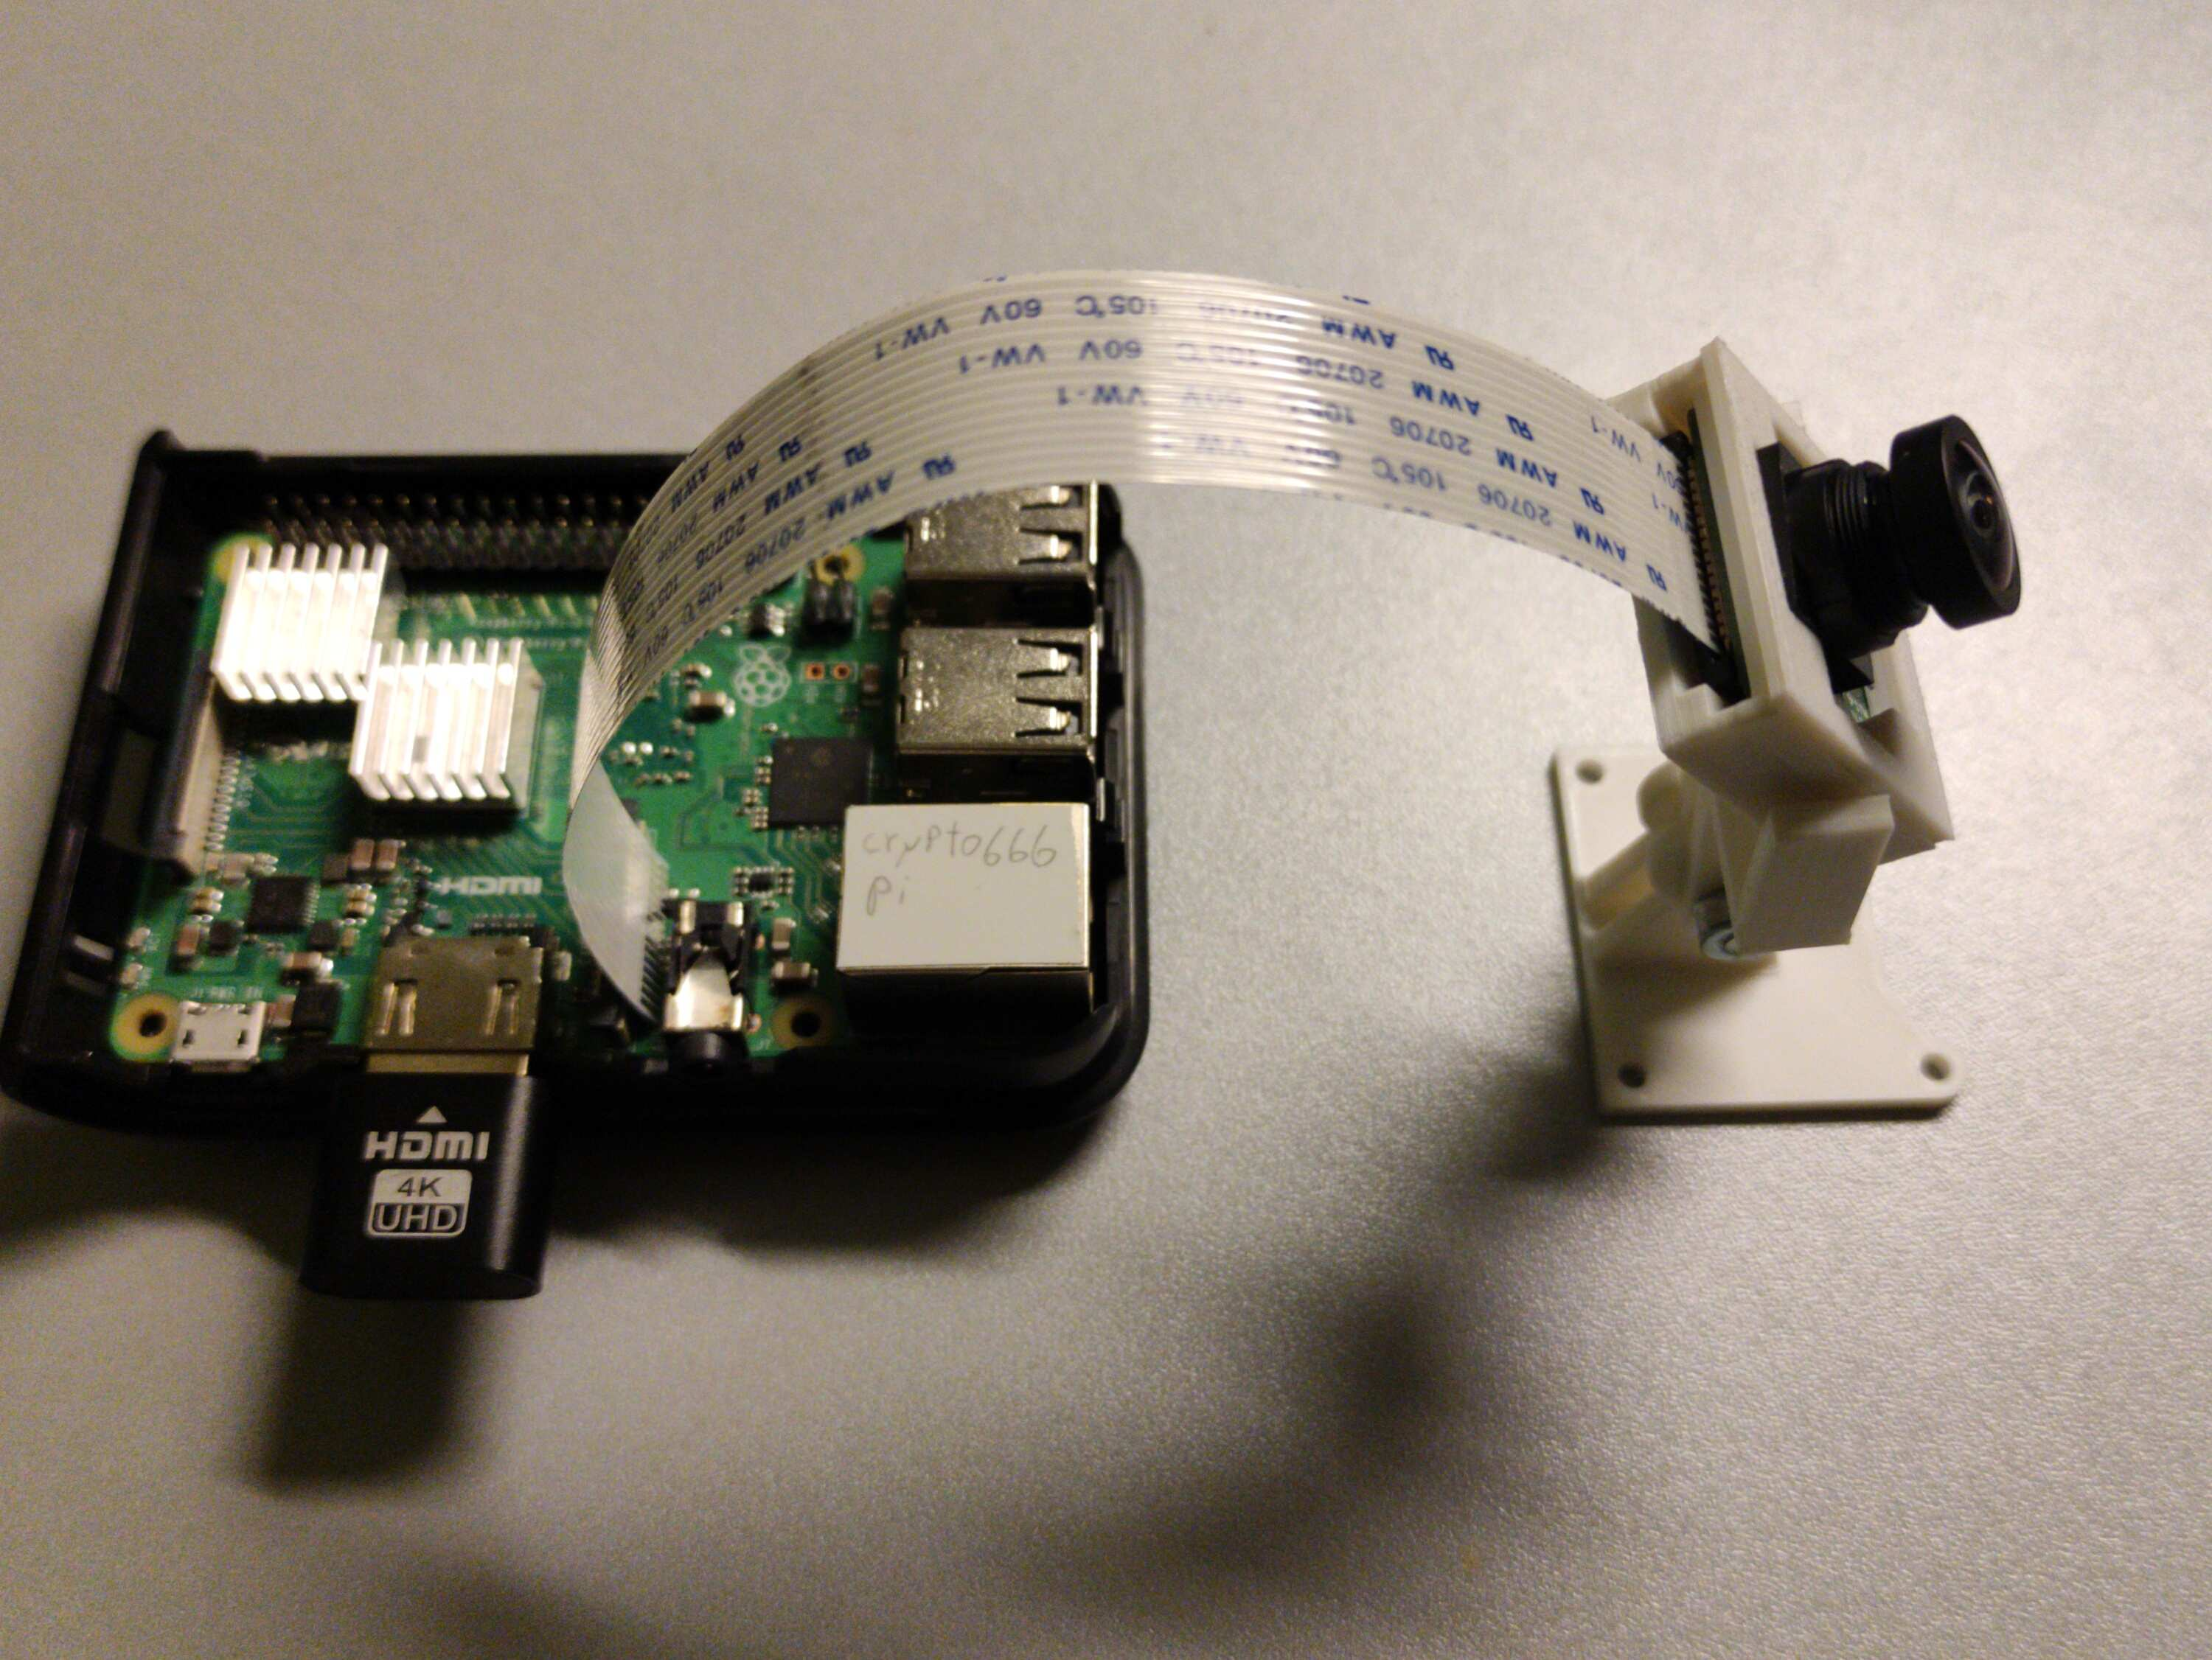
\includegraphics[width=0.8\linewidth]{rPi.jpeg}
	\caption{Raspberry Pi 3B+ and Camera module V2.1}
	\label{fig:raspberry}
\end{figure}

\subsection{Open CV}
OpenCV is an open-source computer vision library suited for video capture and image processing on raspberry pi\cite{3}. We use the latest version 4.5.5. The library offers us a straightforward method of capturing an image from a camera. That is afterwards decoded as \textit{.jpg} format image. Before the very sending of the packet, the \textit{.jpg} is parsed as a byte array. Chunks of size 2$^{16}$-64 bytes are then used as packets for UDP. The subtraction of 64 bytes is used to prevent the UDP frame overflow. Fragments of the code, that performs these actions:

\begin{lstlisting}
MAX = 2**16
MAX_IMG = MAX - 64
...
compressed = cv2.imencode('.jpg', img)[1].tobytes()
count = math.ceil(len(compressed)/(self.MAX_IMG))
array_start = 0
while count:
    array_end = min(size, array_start + self.MAX_IMG)
    self.s.sendto(struct.pack("B", count) + compressed[array_start:array_end], (self.addr, self.port))
    array_start = array_end
    count -= 1
\end{lstlisting}

\subsection{UDP}
User Datagram Protocol (UDP)  is a mechanism based on packet-switching in a computer communication using Internet Protocol (IP)\cite{4}. The idea is to offer the possibility to send messages to other programs with the lowest possible need for protocol management. The main difference between UDP and TCP (Transmission Control Protocol) is that the UDP is not as reliable but is a faster protocol. Redundancy or successful reaching of the destination is not guaranteed. This results in higher stability and speed of the protocol. If you need a reliable transmission, you will probably use TCP\cite{5}. In our solution, the speed of the stream is crucial, so we chose to use the UDP. 

For even greater stability in our solution, we connect the Raspberry Pi with a PC via Ethernet cable and local network. Raspberry Pi has integrated 2.4GHz and 5GHz IEEE 802.11.b/g/n/ac wireless LAN \cite{1} but during experiments, I encountered occasional connection drops when using the wireless connection. We send the packets to the IP address of our computer's ethernet network interface controller. The computer receives the data on the same IP address.

\section{Tracking mechanism}
We are facing the problem of tracking people from the top. After the research described in chapter  \ref{introduction}, we decided to use a tracking mechanism implemented with YOLOv4, DeepSort, and TensorFlow\cite{89}. The YOLOv4 neural network is trained for more types of objects. For example cars. What we want to track is passed to the tracking method as a parameter. Specifically as a list of strings. So we simply add to our list only string containing "person". There are 80 classes you can add, that the neural network will recognize. We need to keep in, that we as well need to perform perspective projection with the received frame. That is because we need to have linear distances between all points in the frame to avoid glitches when rendering spatial audio

\subsection{Neural network setup}
We can run the neural network on a CPU or GPU. GPU has a complex setup and architecture limitations. On the other hand, the CPU has computational limitations. When using the GPU variant, we need to set up the CUDA toolkit. This limits us to use only NVIDIA graphic cards. In our PC we have GeForce GTX 750Ti, which gives us performance comparable with the CPU of our PC, which is Intel Xeon????. 

Our algorithm finds objects using YOLOv4 and then tracks their position using deep sort. We downloaded a pre-trained model for YOLOv4\cite{96}. For faster performance, we can use the \textit{tiny} model, which is less accurate and smaller. This results in a bigger speed of the program. With python script, we convert this model into the corresponding TensorFlow model that will be used in our tracking script.

\subsection{Image perspective transformation}
Our script runs in an infinite loop. In each iteration, it receives a frame from our camera stream described in section \ref{camera}. After the image decoding, we need to perform a perspective transformation to ensure that the frame has uniform distances between points. The OpenCV library offers us a very effective and straightforward way to do this. 

First, we need to find 4 points in our source scene. These points will represent the borders of the output screen. As we are testing this installation at the Institute of Intermedia (IIM) at CTU \cite{95}, I have chosen these points as follows: 1) The bottom points are corners of the camera field of view 2)The upper left point is the corner of the dance floor installed in IIM 3) The upper right point is at the intersection of the dance floor and the camera field of view. We need another four points representing borders into which we want to fit our trimmed source frame. In our case, these will be corners of the 640x480p frame. These two arrays of points are passed to the OpenCV method \textit{getPerspectiveTransform()} which will return a 3x3 transformation matrix. Next, we call the method \textit{warpPerspective()} with our source image, the transformation matrix, and the resolution of the destination image as parameters. 

Finally, this function returns a transformed image. Image as this is ready to be used in the tracking algorithm. The algorithm uses the TensorFlow library to find the objects described in our array mentioned above.

\subsection{Tracking} \label{tracking}
If you wanted to track for example people and cars, you need to modify the array as mentioned above. The recognized objects, that are set up in the array, are then put into the deep sort tracker which returns a list of \textit{tracker} class instances. It gives us the tracked object as a rectangle around the object itself. So we get coordinates of the upper left and bottom right corner in a form of the python tuple data type together with a unique id. We added the computation of coordinates of the tracked person's feet. This was made easily by using the coordinates of the corners as follows

\begin{equation}
\textbf{m}_{(x, y)} = [(l_1 + r_1)/2, (l_2 + r_2)/2],
\end{equation}
where \(\textbf{l}\) is the top left corner and \(\textbf{r}\) is the bottom right corner. We store the \(\textbf{m}\) and a unique id into an instance of a class if an instance holding the same id does not already exist. In that case, we update the coordinates with an interpolation mechanism. This will be described in detail later on.

It is inevitable to encounter situations where the camera stream is blinking, we lose sight of a person, or the tracking mechanism is confused and cannot recognize a person it did recognize in the previous frame. After the first experiments, the neural network with \textit{tiny} model proved it is very good at re-recognizing lost persons. That means, if we start tracking a person and mark it with id 1, lose the person for a few seconds, and then the person reappears, the YOLOv4 will very probably give them the same id. So we try not to forget the last known location of the person by storing it as a value of the class instance. According to tests, we found out that the offset of 6 seconds works best - in most cases it gives the lost person the same id it had before it was lost. 

Another encountered issue was that after finding a person that was lost recently, the tracked location "jumped" from the last known position to the new one. This would appear as an uncomfortable and unrealistic audio glitch in the final spatial mix. I used the same as I did in my previous work, where the same problem appeared. The interpolation update function looks like this:


\begin{lstlisting}
    def update(self, newLocation):
    
        #acceleration is based on the distance between last known and current position
        acceleration = vp.vector(newLocation[0] - self.coord[0], newLocation[1] - self.coord[1], 0)
        
        #'norm' values are values scaled to the size of the frame
        normNewTarget = vp.vector(newLocation[0]/480, newLocation[1]/640, 0)
        normCoord = vp.vector(self.coord[0]/480, self.coord[1]/640, 0)
        normDist = calc_distance(normNewTarget, normCoord)
        
        #Here I do some minimal distance offset
        if sqrt((self.coord[0] - newLocation[0])**2+(self.coord[1] - newLocation[1])**2) < 10:
            #self.coord = newLocation
            return
        else:
            #I change the magnitude of the acceleration according to the size of the distance
            acceleration.mag = 1 + 2*(normDist*20)
        velocity = acceleration
        #I returned 'moved' coordinates of last know position
        self.coord = (int(self.coord[0] + velocity.x), int(self.coord[1] + velocity.y))
\end{lstlisting}
\label{interpolation}
These updated coordinates described in the \textit{update()} function are then used to create the spatial audio mix. This approach performs a smooth interpolation from the last known position to the currently tracked position. The inevitably created latency is inconsiderable. As the neural network can return slightly different results if the person is standing still (we speak about a few pixels), we added the minimal offset to the update function. If the new location changes by less than 10 pixels, we do not perform any update. Otherwise, the tracked point would oscillate around the tracked person even if they were standing still.

\section{Coordinate stream}
Our problem with receiving is that our strategy sends all detected coordinates to every device. So we must determine which the correct coordinates are on the javascript application side. We are adding heuristics to help minimize the mismatch rate of choosing the correct coordinates, which we will describe later.

\subsection{Used communication protocols}
All tracked coordinates in each frame are broadcast locally using Open Sound Control (OSC) protocol to a Processing\cite{94} script and from there to a proxy server using WebSocket protocol. We do so for two reasons. The main is to perform a simple conversion between OSC and WebSocket. Our server script is written in javascript, and it does not natively support OSC. We also did not find any simple way to use WebSocket in python without making it a parallel application. We decided to create a redirection script in Processing. It accepts the OSC packet, parses it as a string, and sends a WebSocket packet to our proxy server. The other reason is readability. The python tracking script should contain only logic maintaining the neural networks and camera stream associated with it.

OSC is mostly described as protocol. However, it does not implement error handling, negotiation, or processing schematics. A better way to describe the OSC is to describe it as a content format. The other is, for example, XML or JSON. Initially, the OSC was implemented for communication between sound synthesizers but found much broader usability. It can be sent via UDP/IP, Ethernet, USB, or Bluetooth but has to be received with another OSC parser\cite{93}.

The WebSocket Protocol enables a form of two-way communication starting with a handshake. It is based on the TCP protocol, and HTTP servers interpret the handshake. The WebSocket protocol is a single TCP connection used in both directions. This approach avoids using HTTP as a bidirectional communication. As HTTP was not implemented to have such a function, using it so would create a variety of problems\cite{92}. 

\subsection{Initial calibration} \label{calibration}
When a user wants to connect to the application for the first time, calibration needs to be undergone. They repeat the exact calibration when the user is lost to the neural network and cannot be found again in time. The web application, which maintains the spatial audio rendering, also handles this calibration.

Firstly, the user needs to stand in the designated calibration area. This area is a circle marked on the floor. The program knows this calibration area as an exact point but checks for any coordinates in a circular vicinity. When the user is in place, he should press the "Calibrate" button in the app. After this, the label changes to "Calibrating" and becomes disabled. During a 5 seconds timeout, the script checks received coordinates and look for one whose distance from the calibration point is less than our offset. If it finds none, or if there are some other coordinates in the vicinity, the calibration will be unsuccessful, and the user shall try it again.

\subsection{Audio rendering}
If the calibration is successful, the program remembers the id associated with that coordinates, and the user will start receiving audio. The app contains a typical play/pause button if the user wants to stop the audio but not the stream. The audio stream will be rendered using the spatial audio engine Resonance Audio. It is initialized with the size of the room, materials from which it consists, and the audio source's coordinates. This setup affects the rendering mechanism accordingly with the real-time received listener coordinates. 

The web application visualizes the room, which appears as a rectangle with three icons. These represent the stationary audio source, calibration point, and the listener's corresponding position in the scene. This visualization is handy for checking if the listener receives coordinates corresponding to his position in the scene. The icon of the calibration point is there to help the user avoid it, if possible, to prevent other users from experiencing unsuccessful calibration.

\subsection{Unsuccessful tracking}
If the web application receives negative coordinates, the tracking mechanism has lost the user from sight for a longer time. If that happens, the app's state returns to "Not Calibrated," which appears on the screen to inform the listener. During this time, the user hears audio with their last known position coordinates, and they should go to the calibration point and calibrate them accordingly to \ref{calibration}.

However, sometimes the tracking mechanism loses the person only for a short time and then assigns it a different id. When this happens, we have an opportunity to prevent the user from the need of re-calibration. We achieve this with a simple heuristic. By remembering the coordinates from the last frame, we can decide if some newly received coordinates with another id could be our coordinates only with a mismatched id. We use a similar approach we have done in the calibration process. If, for example, our last received coordinates were [43, 50], and then the negative coordinate is received, we look into the pack of all received coordinates for all ids. If there are some close to our last known position, e.g. [46, 48], we check if there is no one in the vicinity. If so, we decide that these coordinates are ours and update the id. If not, we cannot assure that we choose correctly, and the user needs to do the calibration again.

\chapter{Testing}

\chapter{Conclusion}

\chapter{Future improvements}

\begin{thebibliography}{1}

 \bibitem{6} M. I. H. Azhar, F. H. K. Zaman, N. M. Tahir and H. Hashim, "People Tracking System Using DeepSORT," 2020 10th IEEE International Conference on Control System, Computing and Engineering (ICCSCE), 2020, pp. 137-141, doi: 10.1109/ICCSCE50387.2020.9204956.

 \bibitem{98} Silent Disco: A Popular Trend that Has Been Out For Years, (2022), The Silent Disco Company, https://thesilentdiscocompany.co.uk/blog/silent-disco-history/
 
 \bibitem{99} Cambridge Dictionary, Cambridge University Press (2022), https://dictionary.cambridge.org/dictionary/english/public-address-system
 
 \bibitem{97} GitHub repository, vilijonak/Bachelor-thesis/Semester Work, (2021) https://github.com/vilijonak/Bachelor-thesis/tree/main/Semester%20Work
 
 \bibitem{96} GitHub Repository, theAIGuysCode/yolov4-deepsort: Object tracking implemented with YOLOv4. DeepSort, and TensoFlow (2021), https://github.com/theAIGuysCode/yolov4-deepsort

\bibitem{95} Bittner, Jiri, and Jiri Zara. "DCGI Laboratories at CTU Prague."

\bibitem{94} Reference / Processing.org, Fry, Ben and Reas, Casey (2004), https://processing.org/reference 

\bibitem{93} Freed, Adrian, and Andrew Schmeder. "Features and Future of Open Sound Control version 1.1 for NIME." NIME. Vol. 4. No. 06. 2009.

\bibitem{92} Fette, Ian, and Alexey Melnikov. "The websocket protocol." (2011).

\bibitem{91} Resonance Audio, Resonance Audio - Fundamental Concepts, https://resonance-audio.github.io/resonance-audio/discover/concepts.html

\bibitem{90} D. Y. N. Zotkin, J. Hwang, R. Duraiswaini and L. S. Davis, "HRTF personalization using anthropometric measurements," 2003 IEEE Workshop on Applications of Signal Processing to Audio and Acoustics (IEEE Cat. No.03TH8684), 2003, pp. 157-160, doi: 10.1109/ASPAA.2003.1285855.

\bibitem{89} GitHub Repository, theAIGuysCode/yolov4-deepsort: Object tracking implemented with YOLOv4, DeepSort, and Tensorflow (2020), https://github.com/theAIGuysCode/yolov4-deepsort

 \bibitem{1} Raspberry Pi Documentation: Raspberry Hardware (2022), https://www.raspberrypi.com/documentation/computers/raspberry-pi.html

 \bibitem{2} Raspberry Pi Documentation: Camera, (2022), https://www.raspberrypi.com/documentation/accessories/camera.html
 
 \bibitem{3} OpenCV: OpenCV modules, Doxygen, 2021, https://docs.opencv.org/4.5.5/
 
 \bibitem{4} Postel, Jon. "User datagram protocol." (1980).
 
 \bibitem{5} Xylomenos, George, and George C. Polyzos. "TCP and UDP performance over a wireless LAN." IEEE INFOCOM'99. Conference on Computer Communications. Proceedings. Eighteenth Annual Joint Conference of the IEEE Computer and Communications Societies. The Future is Now (Cat. No. 99CH36320). Vol. 2. IEEE, 1999.



\end{thebibliography}

\end{document}

